\documentclass{standalone}
\usepackage{tikz}
\begin{document}
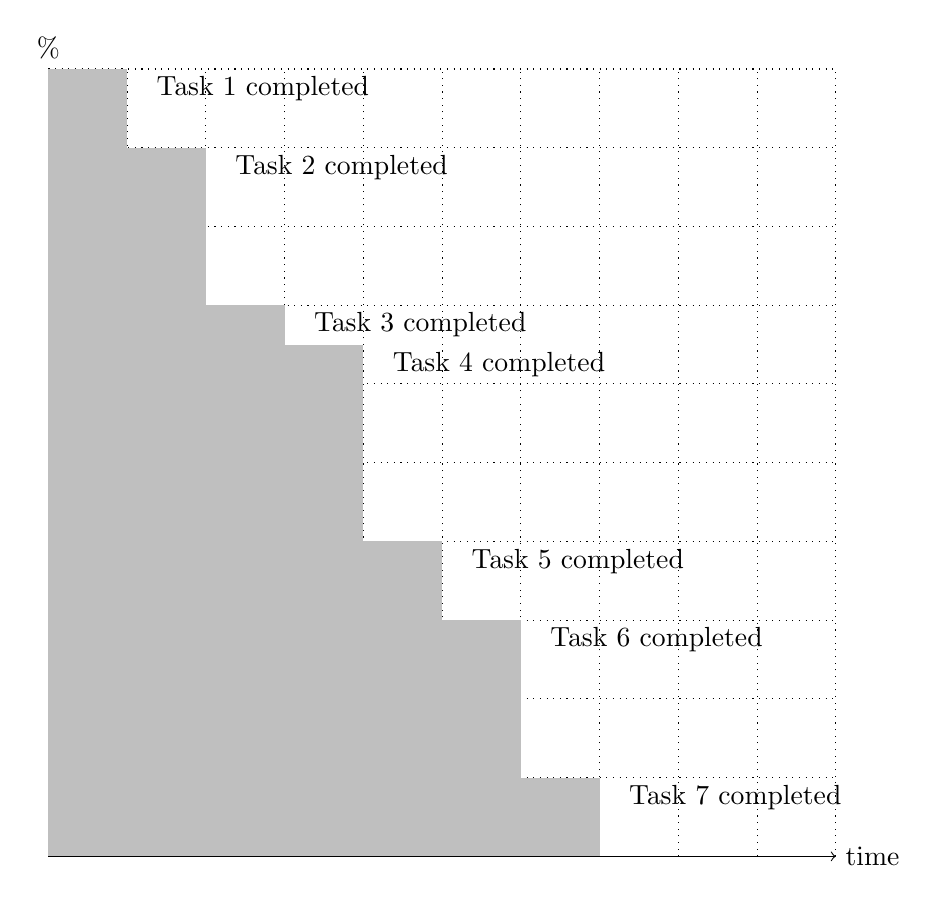
\begin{tikzpicture}
    \draw[step=1.0,black,dotted] (0,0) grid (10,10);
    \draw[->] (0,0) -- (10,0) node[right] {time};
    \draw (0,0) -- (0,10) node[above] {\%};
    \foreach [count=\x] \y in {10,9,7,6.5,4,3,1}
        {
        \path[fill=gray!50] (\x-1,0) rectangle (\x,\y) ;
        \node[anchor=west] at (\x+0.25,\y-0.25) {Task \x\ completed};
        }
    
\end{tikzpicture}
\end{document}